\documentclass[11pt]{article}
\usepackage{amsmath,amssymb}
\usepackage{lmodern}
\usepackage{cite}
\usepackage{listings}
\usepackage{graphicx}
\usepackage{minted}
\usepackage{url}
\usepackage{hyperref}

\title{sympy-nondim}
\author{Christoph Heindl \\ \url{https://github.com/cheind} }
\date{\today}

\begin{document}
\maketitle

\section{Introduction}
This Python package addresses physical dimensional analysis. In particular, \texttt{sympy-nondim} calculates from an unknown relation of (dimensional) variables, a new relation of (usually fewer) dimensionless variables.

\section{Example}
Suppose that you are asked to find an equation for the period of a simple frictionless pendulum (example taken from \cite{lemons2017student}). Unaware of the solution, you may assume that the period $t$ of the pendulum depends somehow on the (massless) string length $l$, the point mass $m$, the initial release angle $\theta$ and gravitational acceleration $g$ as shown in the following diagram.
\begin{center}
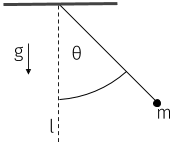
\includegraphics[width=0.3\textwidth]{pendulum.png}
\end{center}
Hence, you need to find an unknown relation $$t = f(l,m,g,\theta).$$ You plan to carry out experiments to study the value of $t$ for different values of all the independent variables in various combinations. Assuming $N$ values per variable, you will perform on the order of $N^4$, i.e $10,000$ experiments when $N=10$. 

Using dimensional analysis we can a) reduce the number of experiments and b) gain insights into the unknown functional relationship of the variables. Dimensional analysis applies the principle dimensional homogeneity to manipulate a functional relationship of dimensional variables $$y = f(a,b,c,...)$$ into a new function $F$ of (usually fewer) nondimensional variables $$Y = F(A,B...).$$

\subsection{Problem setup}
In the pendulum case we first define the relevant symbols, their dimensions, and define the abstract equation we would like to analyze.
\begin{minted}{python}
import sympy
from sympy.physics import units

t, m, l, g, theta = sympy.symbols('t m l g theta')
dimmap = {
    t:units.time, 
    m:units.mass, 
    l:units.length, 
    g:units.acceleration, 
    theta:units.Dimension(1)
}

eq = sympy.Eq(t, sympy.Function('f')(m,l,g,theta))
print(sympy.latex(eq))
\end{minted}
$$t = f{\left(m,l,g,\theta \right)}.$$

\subsection{Result}
Next, we apply dimensional analysis
\begin{minted}{python}
import nondim

r = nondim.nondim(eq, dimmap)
print(sympy.latex(r))
\end{minted}
Which returns a new equation
\begin{equation}
    \sqrt{\frac{g}{l}}t = F{\left(\theta \right)}. \label{eq:A}
\end{equation} Note, all variable products appearing on the LHS and RHS are dimensionless. Solving for $t$ yields
\begin{minted}{python}
f = sympy.Eq(t, sympy.solve(r, t)[0])
print(sympy.latex(f))
\end{minted}
$$t = \sqrt{\frac{l}{g}}F{\left(\theta \right)}.$$ 
Dimensional analysis provides us with the following valuable insights
\begin{enumerate}
    \item The mass $m$ is irrelevant in the given problem.
    \item There is no need to consider an unknown function $f$ of four independent variables, instead we can reduce the search to unknown function $F$ of a single variable (initial release angle $\theta$). Few experiments according to Equation~\ref{eq:A} will quickly reveal that $F(\theta)\approx 2\pi$ for small angles.
    \item Keeping $F{\left(\theta \right)}$ constant, the period $t \propto  \sqrt{\frac{l}{g}}$.
\end{enumerate}

To learn more about dimensional analysis and how it might be helpful, consider \cite{szirtes2007applied, santiago2019first, sonin2001dimensional, lemons2017student,schetz1999fundamentals}. The method implemented in this library is based on the Buckingham-Pi theorem and the Rayleigh algorithm as explained in \cite{szirtes2007applied}. The method implemented here frames the problem in linear algebra terms, see \texttt{buckpi.py} for details.

\section{Mathematical Notes}
A dimensional equation of $N_v$ variables
\begin{equation}
    f(x_1,x_2,\ldots,x_{N_v-1}) = x_{N_v} \label{eq:fnc}
\end{equation}
is dimensionally homogeneous, if it can be written as
\begin{equation}
    g(\pi_1,\pi_2,\ldots,\pi_{N_p}) = 0.
\end{equation}
Here $\left\{\pi_1,\pi_2,\ldots,\pi_{N_p}\right\} = \Pi$ is a complete (and independent) set of $|\Pi|={N_p}$ dimensionless variable products. 

Without loss of generality, consider 3 variables $x,y,z$. Let $\left[\cdot\right]$ denote the dimension, we require
\begin{align}
    \left[\pi_i\right] &= \left[x^{\alpha_i}y^{\beta_i}z^{\gamma_i} \right] \\
    &=\left[x^{\alpha_i}\right]\left[y^{\beta_i}\right]\left[z^{\gamma_i}\right] \\
    &=\left[x\right]^{\alpha_i}\left[y\right]^{\beta_i}\left[z\right]^{\gamma_i} = 1 \label{eq:pi}    
\end{align}
for unknown rational scalars $\left\{\alpha_i,\beta_i,\gamma_i\right\}.$ In a dimensional system, each dimension is defined as product of $N_k$ base-dimensions. Assuming base-dimensions mass $M$, length $L$ and time $T$, we write 
\begin{equation}
    \left[x\right] = M^mL^lT^t, \label{eq:xinmlt}
\end{equation}
where the values of the scalars $\left\{m,l,t\right\}$ depend variable dimension. For example, gravitational acceleration $g$ in the $MLT$-system is given by
\begin{equation}
    \left[g\right] = M^0L^1T^{-2}.
\end{equation}

\subsection{Physical dimensions as vector spaces}
Physical dimensions form a commutative (abelian) group $G$ under multiplication~\cite{wiki:Dimensional_analysis}: if $M,L \in G$, then $M^m,L^l \in G,$ assuming $m,l \in \mathbb{Q}$ and also $M^m \times L^l \in G$. The identity is $1 = M^0$.

The group $G$ can be described as a vector space over the field of rational numbers, mapping $[x] = M^0L^1T^{-2}$ to $(0,1,-2)^T$. Dimensional multiplication corresponds then to vector addition and scalar multiplication to raising dimensional symbols to a rational power. The basis is spanned by $N_k$ canonical unit directions corresponding to the physical base dimensions. For example, mass $M$ is mapped to $(1,0,0)^T$ in a three-dimensional vector space associated with the base dimensions $MLT$. The origin $\mathbf{0}$ of the vector space $(0,0,0)^T$ corresponds to a dimensionless quantity.

Using vector notation, we may rewrite Equation~\ref{eq:xinmlt}
\begin{equation}
    \alpha_i[x] + \beta_i[y] + \gamma_i[z] = \mathbf{0}, \label{eq:zeroeq}
\end{equation}
where we assume that $\left[\cdot\right]$ returns the vector space mapping of the variable's dimensions. 

\subsection{Determining $\pi$}

We may rewrite Equation~\ref{eq:zeroeq} as a matrix-vector product
\begin{equation}
    \mathbf{D}\mathbf{v} =\begin{pmatrix}[x] & [y] & [z]\end{pmatrix}\begin{pmatrix} \alpha_i \\ \beta_i \\ \gamma_i\end{pmatrix} = \mathbf{0},
\end{equation}
where $\mathbf{D}$ is the $N_k \times N_v$ dimensional matrix. Hence, determining $\Pi$ becomes equivalent to the problem of finding a set of vectors $\mathbf{v}$ for which
\begin{equation}
    \mathbf{D}\mathbf{v}=\mathbf{0}.
\end{equation}
The set of vectors $\{\mathbf{v} \mid \mathbf{D}\mathbf{v}=\mathbf{0}\}$ span a sub-space of the domain of the linear map $\mathbf{D}$: the null-space. The dimensionality of the null-space is given by the rank-nullity theorem
\begin{equation}
    N_p = N_v - \text{rank}(\mathbf{M}) = \text{nullity}(\mathbf{M}) = |\Pi|,
\end{equation}
and determines the number of independent dimensionless products. The span of the null-space is not unique and this leads potentially different $\Pi$ sets. For practical purposes one should try to find a basis in which variables of interest will appear in only one of the $\pi$ terms. That's always possible as long of the variables of interest are 'free' variables. 

\subsection{Specific solutions}
When the non-dimensionalization of Equation~\ref{eq:fnc} results in a single $\pi$ term
\begin{equation}
    g(\pi_1) = 0,
\end{equation}
then $\pi_1$ is a root of $g$. Assuming $g$ has only a single root (or discrete number of them), we see $\pi_1$ itself must be an (unknown) constant
\begin{equation}
    \pi_1 = c.
\end{equation}
When $g$ is a function of more than one dimensionless product
\begin{equation}
    g(\pi_1, \pi_2) = 0,
\end{equation}
we may invoke the Implicit Function Theorem to solve for one of the arguments and write instead
\begin{equation}
    \pi_1 = h_1(\pi_2).
\end{equation}
Similarly for three arguments $g(\pi_1, \pi_2, \pi_3) = 0$ we have
\begin{equation}
    \pi_1 = h_2(\pi_2, \pi_3).
\end{equation}

\subsection{References}
\bibliographystyle{alpha}
\begingroup
\renewcommand{\section}[2]{}%
\bibliography{biblio}
\endgroup

\end{document}
